\begin{figure}[H]
    \centering
    \caption{Exemplo de árvore de decisão para classificação binária.}
    \label{fig:arvore}
    \scalebox{0.8}{
        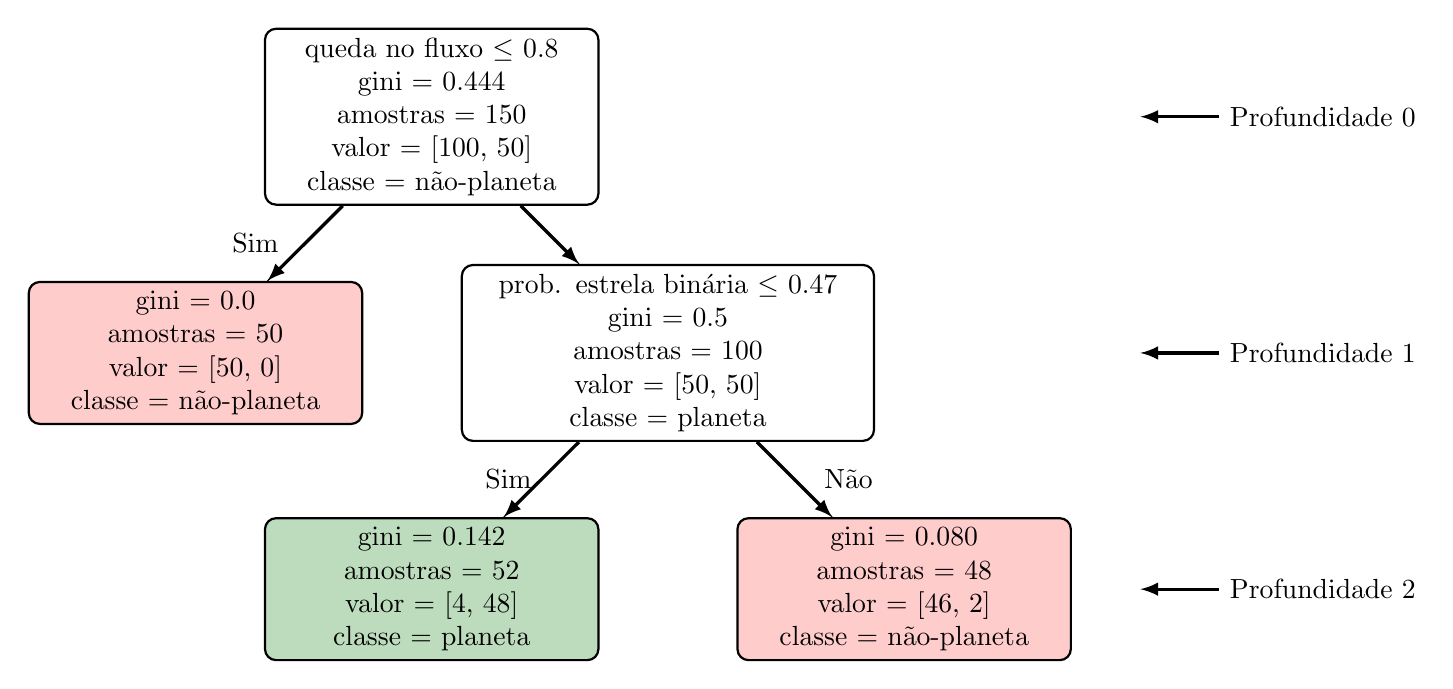
\begin{tikzpicture}
        \tikzstyle{bloco} = [rectangle, draw=black, thick, text width = 4cm, text centered, rounded corners]
        
        \node [bloco] (raiz) {queda no fluxo $\leq$ 0.8 \\
               gini = 0.444 \\
               amostras = 150 \\
               valor = [100, 50] \\
               classe = não-planeta}
            [level distance = 3cm, sibling distance = 6cm]
            child {node (np1) [bloco, fill=red!20] {gini = 0.0 \\
               amostras = 50 \\
               valor = [50, 0] \\
               classe = não-planeta}
                    edge from parent
                        node[left]{Sim \textcolor{white}{.}}
               }
            child {node (ramo) [bloco, text width = 5cm] {prob. estrela binária $\leq$\ 0.47 \\
               gini = 0.5 \\
               amostras = 100 \\
               valor = [50, 50] \\
               classe = planeta}
                child {node (pc) [bloco, fill=ForestGreen!30] {gini = 0.142 \\
                    amostras = 52 \\
                    valor = [4, 48] \\
                    classe = planeta}
                        edge from parent
                            node[left]{Sim}
                    }
                child {node (np2) [bloco, fill=red!20] {gini = 0.080 \\
                    amostras = 48 \\
                    valor = [46, 2] \\
                    classe = não-planeta}
                        edge from parent
                            node[right]{\textcolor{white}{.} Não}
                    }
               };
            \draw[-latex, very thick] (raiz) -- (np1);
            \draw[-latex, very thick] (raiz) -- (ramo);
            \draw[-latex, very thick] (ramo) -- (pc);
            \draw[-latex, very thick] (ramo) -- (np2);
            
            \draw[latex-, very thick] (9, 0) -- (10, 0) node[right]{Profundidade 0};
            \draw[latex-, very thick] (9, -3) -- (10, -3) node[right]{Profundidade 1};
            \draw[latex-, very thick] (9, -6) -- (10, -6) node[right]{Profundidade 2};
        \end{tikzpicture}
    }
    \caption*{\small Fonte: Elaboração própria.}
\end{figure}